\subsection{Preprocesamiento de imágenes}

El preprocesamiento de las imágenes del conjunto de datos se divide en dos etapas: la estandarización de las imágenes y el aumento de datos.

La estandarización consiste en garantizar que todas las imágenes del dataset cumplan con el formato de entrada requerido por EfficientNet-B3. Como se establece en la RN-09, la resolución estándar es de $300 \times 300$ píxeles, por lo que todas las imágenes fueron redimensionadas a esta resolución y convertidas al formato JPG. Adicionalmente, los valores de píxel se normalizan en el rango $[0,1]$ dividiendo entre 255, lo cual es una práctica estándar para estabilizar el entrenamiento de redes neuronales profundas.

La segunda etapa corresponde al aumento de datos o \textit{data augmentation}, que consiste en aplicar transformaciones aleatorias sobre las imágenes durante el entrenamiento con el objetivo de que el modelo aprenda a generalizar ante la variabilidad visual presente en las capturas de campo. A diferencia de la estandarización, estas transformaciones no se aplican sobre el dataset almacenado en disco sino en tiempo real durante el entrenamiento, mediante capas de aumento integradas directamente en el modelo con \texttt{tf.keras.layers}.

Las transformaciones seleccionadas para las imágenes de corteza son las siguientes:

\begin{itemize}
    \item \textbf{Flip horizontal y vertical}: dado que las fotografías de corteza pueden tomarse desde cualquier ángulo en campo, los patrones de galerías e indicios de infestación son igualmente reconocibles en cualquier orientación.
    \item \textbf{Rotaciones}: por la misma razón anterior, se aplican rotaciones de hasta 90° para simular diferentes ángulos de captura. \item \textbf{Variaciones de brillo y contraste}: simulan las distintas condiciones de iluminación natural presentes durante las jornadas de captura en el bosque.
    \item \textbf{Zoom leve}: simula variaciones en la distancia de captura respecto al tronco del árbol.
\end{itemize}

\begin{figure}[H]
    \centering
    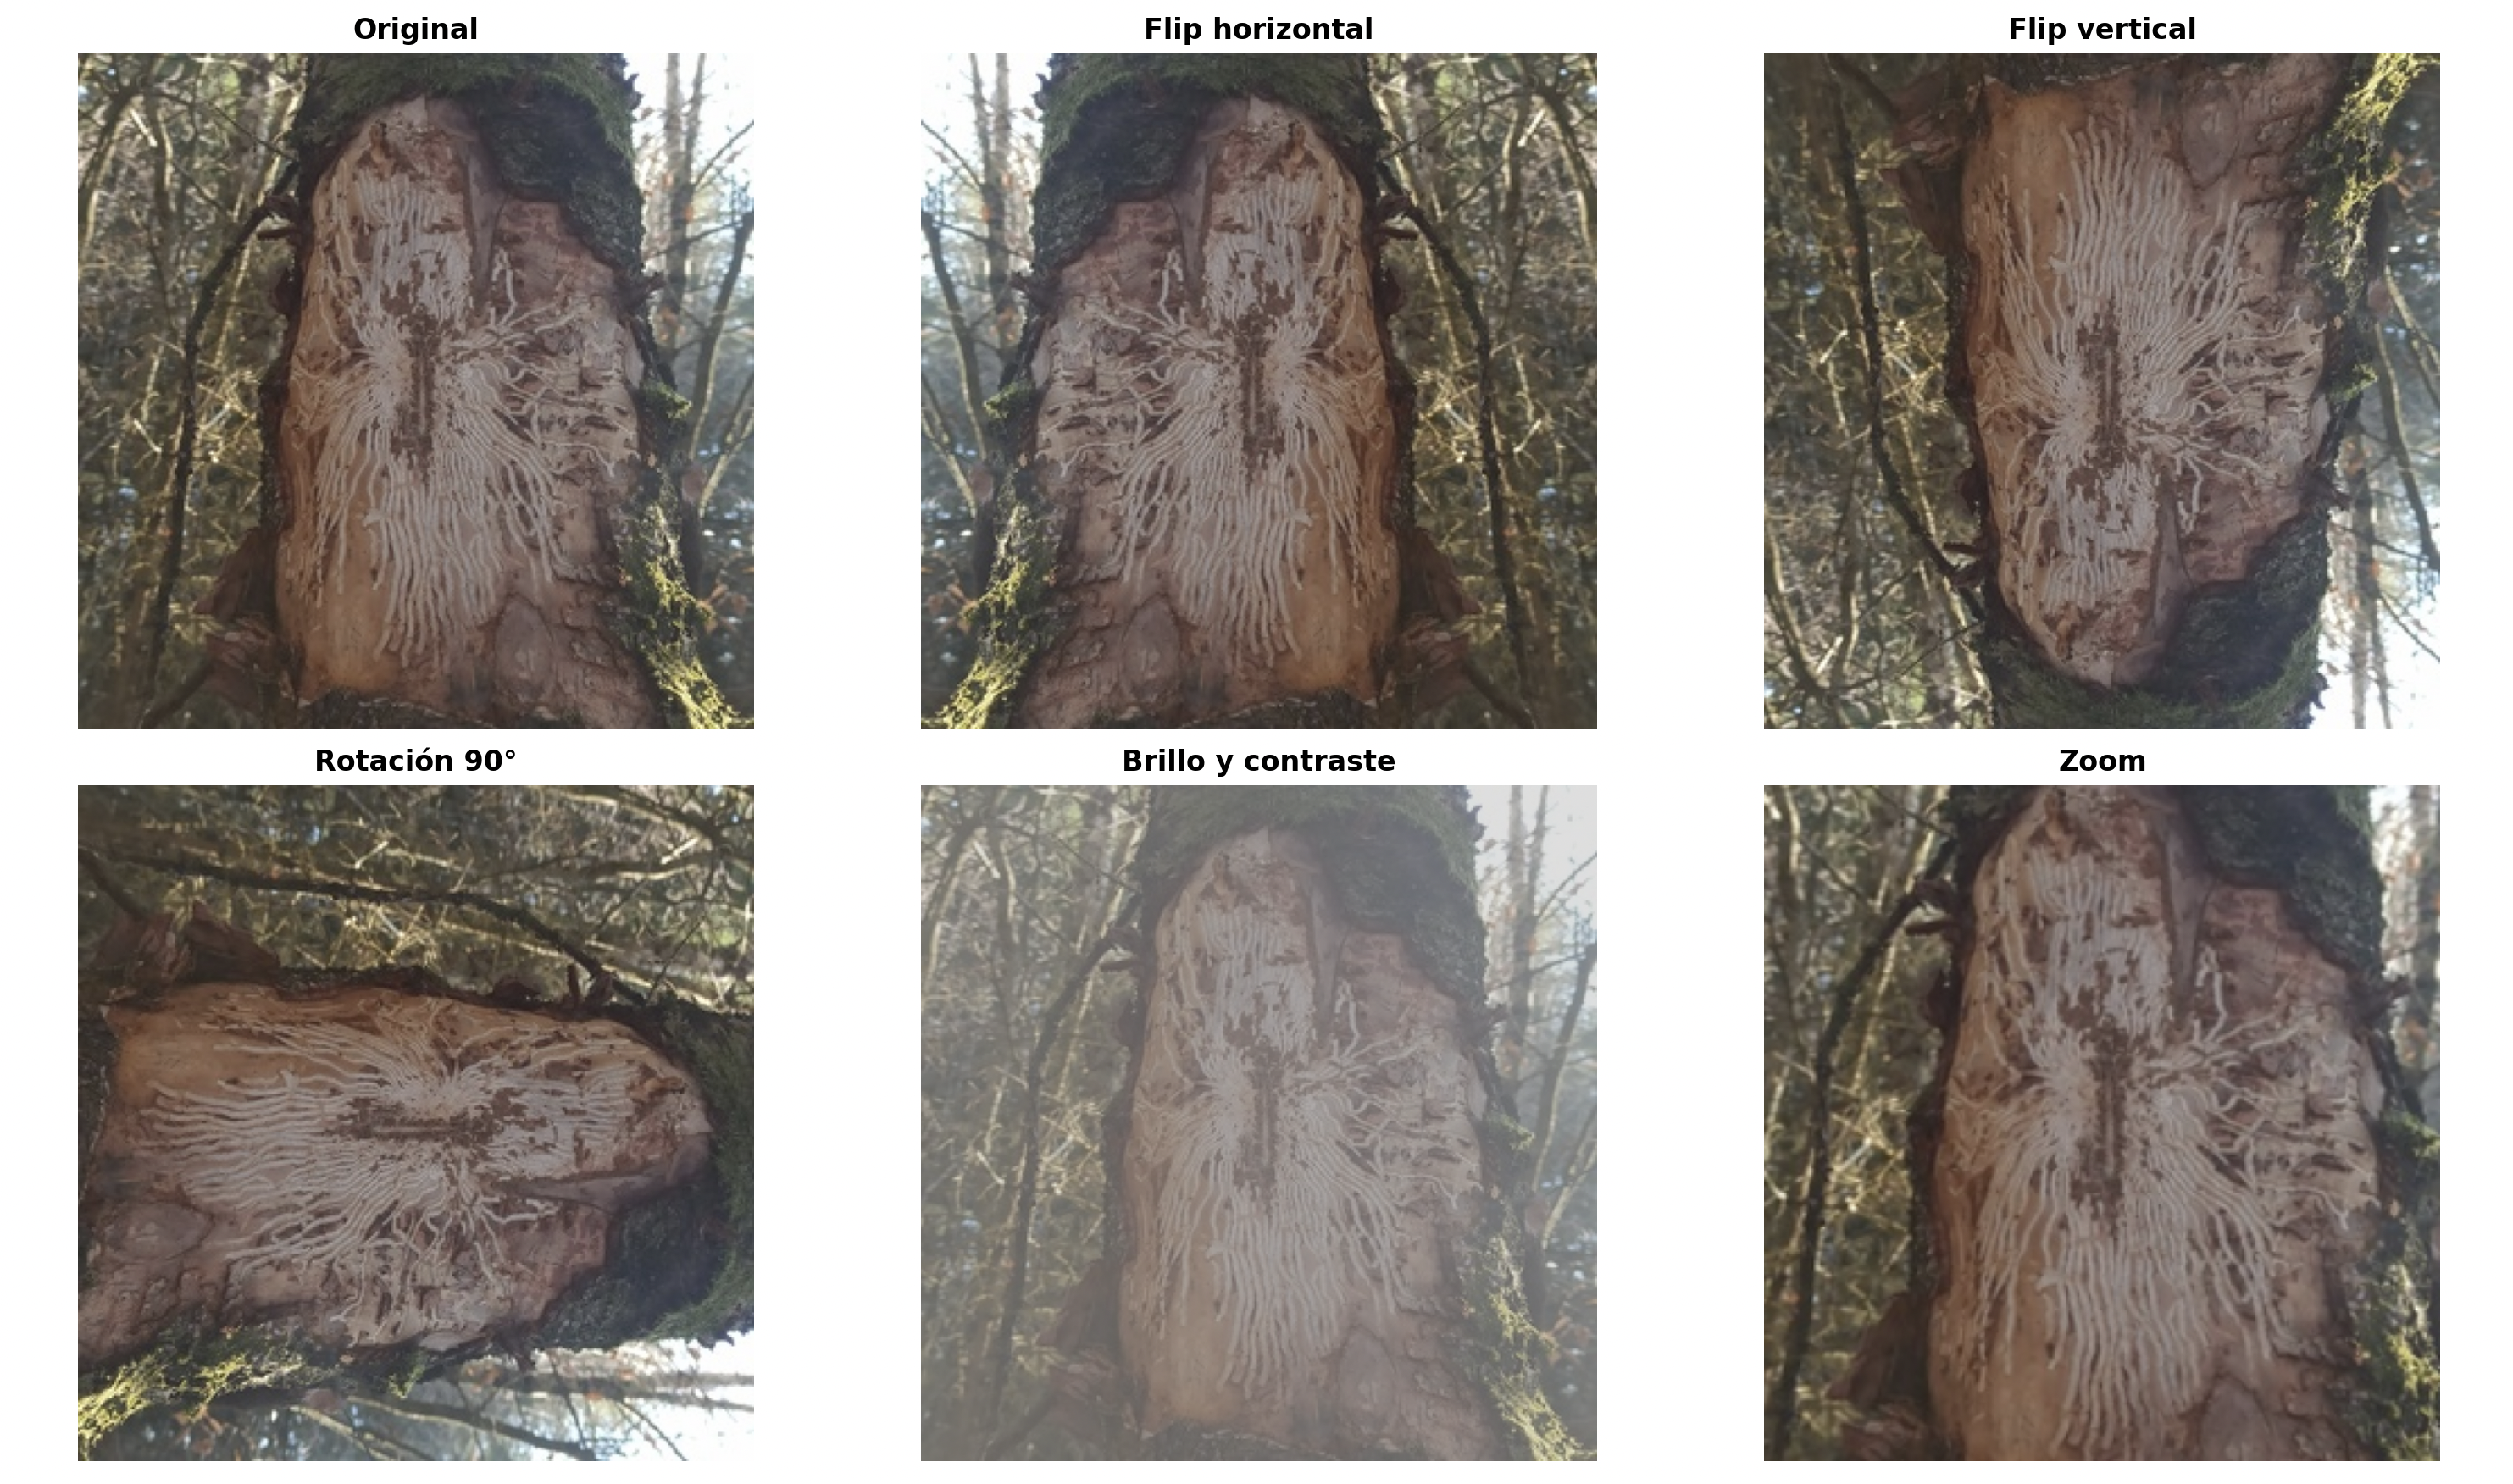
\includegraphics[width=0.8\textwidth]{images/C6/dataAugmentation.png}
    \caption{Muestra de configuración de ajustes de una misma imagen.}
    \label{fig:dataAugmentation}
\end{figure}

No se aplican deformaciones fuertes ya que los patrones generados por las larvas en la corteza podrian perderse en el proceso, afectando de manera negativa el aprendizaje del modelo.